%%%%%%%%%%%%%%%%%%%%%%%%%%%%%%%%%%%%%%%%%%
\section{Esperimenti}
\frame{\frametitle{Ciclo di lavoro}
\centering
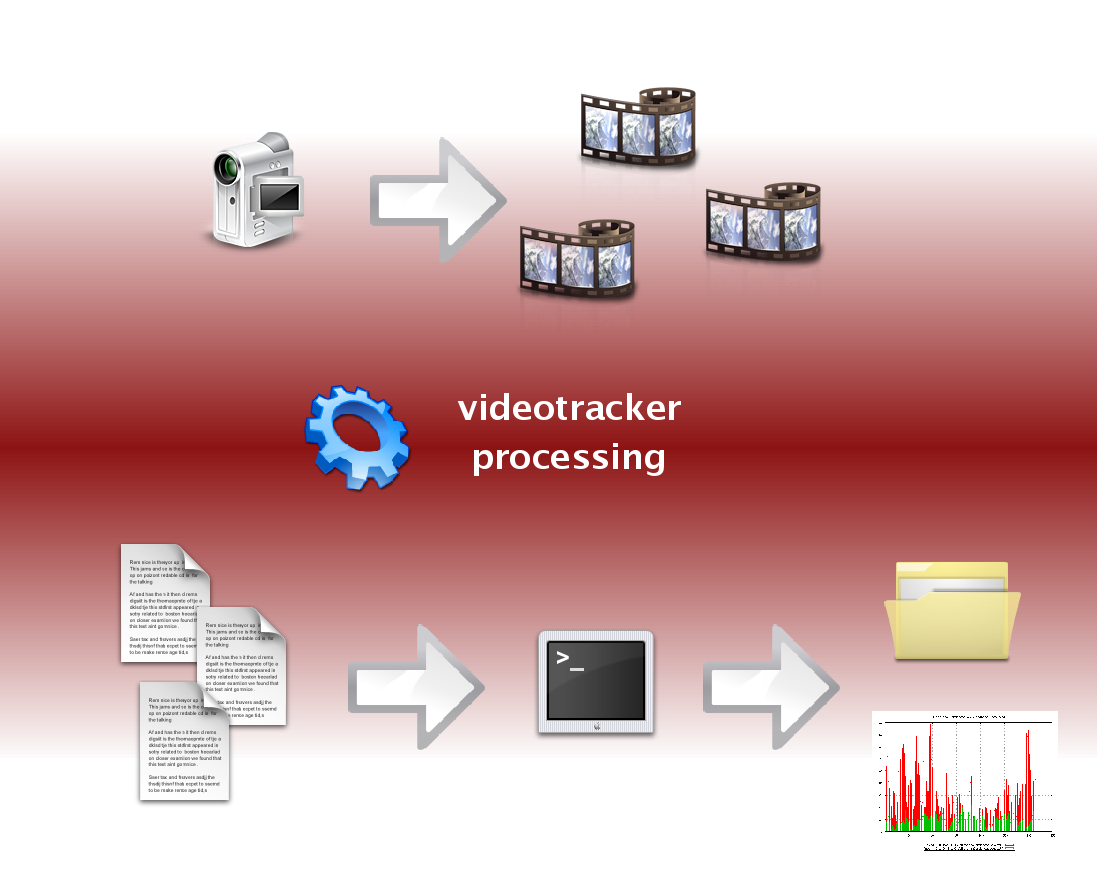
\includegraphics[scale=0.35]{img/Presentazione.png}

}

%%%%%%%%%%%%%%%%%%%%%%%%%%%%%%%%%%%%%%%%%%
\frame{\frametitle{Parametri degli esperimenti}
\begin{block}{}\begin{small}\alert{\textbf{Esperimenti}}: variazione di tre parametri nei tre video selezionati \end{small}\end{block}
\pause
\begin{footnotesize}\begin{description}
\item [\textbf{Intervallo Frames}] Frames tra due applicazioni consecutive del Tracking\\Distanziare nel tempo due applicazioni successive di \alert{Tracking} consente di peggiorare il lavoro del filtro di Kalman\pause
\item [\textbf{Q - Area Kalman}] Autovalori della matrice del rumore sul processo (Q)\\Ririsulta l'area di confidenza del filtro di \alert{Kalman}, ovvero l'area nella quale deve risiedere il blob al frame precedente per poter continuare ad essere tracciato all'esecuzione successiva.\pause
\item [\textbf{Samples ConDensation}] Numero dei samples ad ogni esecuzione\\ \`E il numero totale di samples che utilizza il \alert{ConDensation} per effettuare i calcoli statistici ad ogni esecuzione del Tracking
 \end{description}\end{footnotesize}

}
%%%%%%%%%%%%%%%%%%%%%%%%%%%%%%%%%%%%%%%%%%
\frame{\frametitle{Output \& Scripting}
\begin{block}{}
\begin{small}Il software produce sei files di output:\end{small}
\begin{scriptsize}\begin{description}
\item [\textit{coordinateReali.txt}] Coordinate reali dell'oggetto da tracciare
\item [\textit{coordinateKalman.txt}] Coordinate previste da Kalman
\item [\textit{coordinateCondensation.txt}] Coordinate previste dal ConDensation
\item [\textit{distanzaKalman.txt}] \alert{$\delta_k$} Distanza tra le coordinate reali e la previsione di Kalman
\item [\textit{distanzaCondensation.txt}]\alert{$\delta_c$} Distanza tra coord reali e previsione ConDensation
\item [\textit{Risultati.txt~~~~~~~~~~~}]  distanza media, $\overline{\delta}_k, \overline{\delta}_c$, varianza media ConDensation ($\overline{\sigma}_x, \overline{\sigma}_y$).
 \end{description}\end{scriptsize}
\end{block}
\pause
\begin{small}I files ottenuti vengono processati da due \alert{script bash}\end{small}
\begin{scriptsize}\begin{description}
\item [\textbf{gplot.sh}] Invoca degli script \alert{GNUPlot} che restituiscono dei grafici relativi ai risultati ottenuti, consentendo una valutazione immediata dell'esperimento effettuato.
\item[\textbf{exp.sh}] Organizza i files di output e le immagini comparative disegnate nel filesystem, consentendo un facile \alert{riepilogo} dei risultati ed una ordinata catalogazione di questi.
 \end{description}\end{scriptsize}
}
%%%%%%%%%%%%%%%%%%%%%%%%%%%%%%%%%%%%%%%%%%
\subsection{Video}

\frame{\frametitle{Video selezionati}
\hrulefill
\begin{columns}
\column{.30\textwidth}\centering
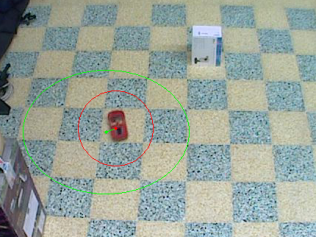
\includegraphics[scale=0.21]{img/movie12.png}

\column{.70\textwidth}
\begin{footnotesize}\begin{enumerate}
\item [1] \textbf{movie12.mjpeg} (mjpeg/xvid)
	\begin{itemize}
	\item occlusione, moto circolare e costante
	\item 640x480, 25$fps$, 50.4$s$\end{itemize}
\end{enumerate}\end{footnotesize}
\end{columns}

\hrulefill \pause

\begin{columns}
\column{.70\textwidth}
\begin{footnotesize}\begin{enumerate}
\item[2] \textbf{tappeto\_nozoom.avi} (avi/xvid)
	\begin{itemize}
	\item moto vario, repentine accelerazioni, oggetto entra ed esce dalla scena
	\item 320x240, 10$fps$, 59$s$\end{itemize}
\end{enumerate}\end{footnotesize}
\column{.30\textwidth}\centering
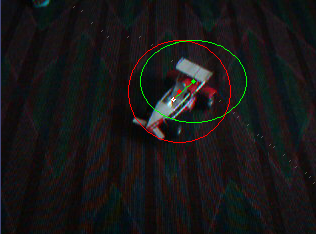
\includegraphics[scale=0.21]{img/tappetonozoom.png}
\end{columns}

\hrulefill \pause

\begin{columns}
\column{.30\textwidth}\centering
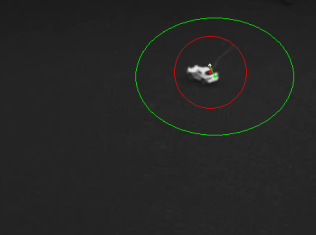
\includegraphics[scale=0.21]{img/singlecar.png}
\column{.70\textwidth}
\begin{footnotesize}\begin{enumerate}
\item[3] \textbf{singlecar.avi} (avi/xvid)
	\begin{itemize}
	\item moto costante, oggetto entra ed esce dalla scena
	\item 648x484, 30$fps$, 33$s$\end{itemize}
\end{enumerate}\end{footnotesize}
\end{columns}
\hrulefill
}


% \frame{\frametitle{Primo video - movie12.mjpeg}
% \begin{columns}
% \column{.65\textwidth}
% \begin{small}\begin{itemize}
%  \item occlusione, moto circolare e costante
% \item 640x480, 25$fps$, 50.4$s$
% \end{itemize}\end{small}
% 
% \column{.35\textwidth}\centering
% 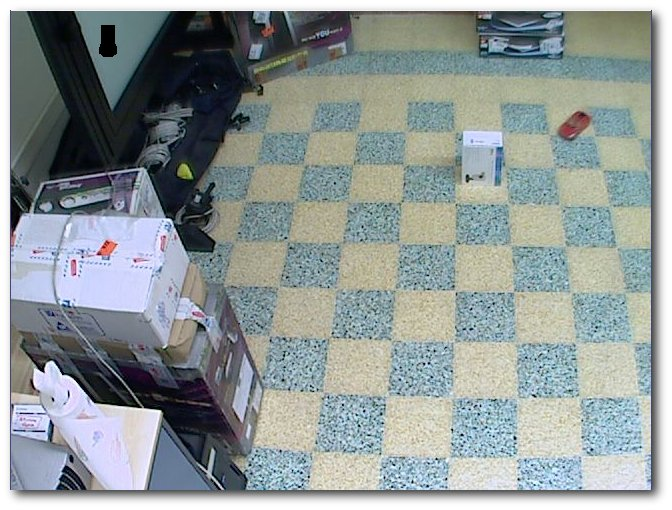
\includegraphics[scale=0.15]{../relazione/figure/movie12.jpg}
% \end{columns}
% \begin{columns}
% 
% \column{.20\textwidth}
% \begin{scriptsize}
% \begin{itemize}
% \item [M]3
% \item [Q]1000
% \item [S]1000
% \end{itemize}
% \end{scriptsize}
% 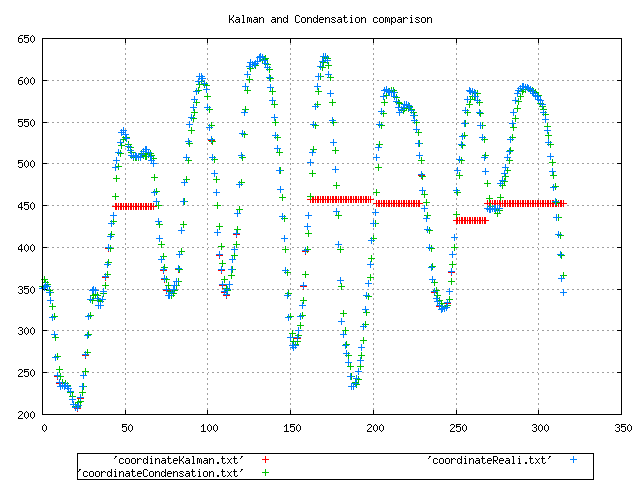
\includegraphics[scale=0.1]{../esperimenti/movie12/mod_3-Q_1000-S_1000/plot.png}\\
% 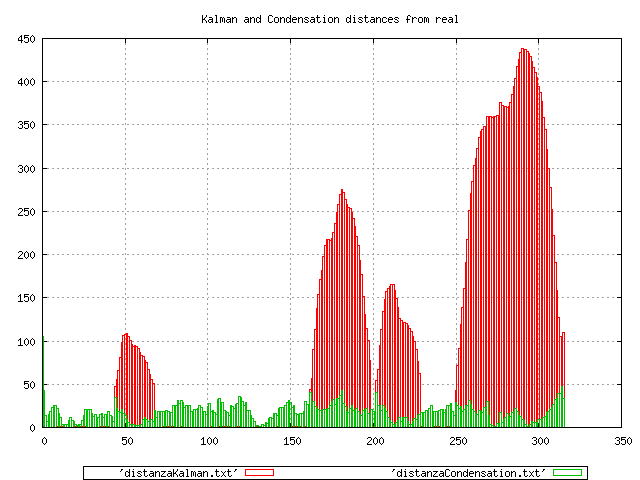
\includegraphics[scale=0.1]{../esperimenti/movie12/mod_3-Q_1000-S_1000/plot-distances.png}
% 
% \column{.20\textwidth}
% \begin{scriptsize}
% \begin{itemize}
% \item [M]3
% \item [Q]2000
% \item [S]1000
% \end{itemize}
% \end{scriptsize}
% 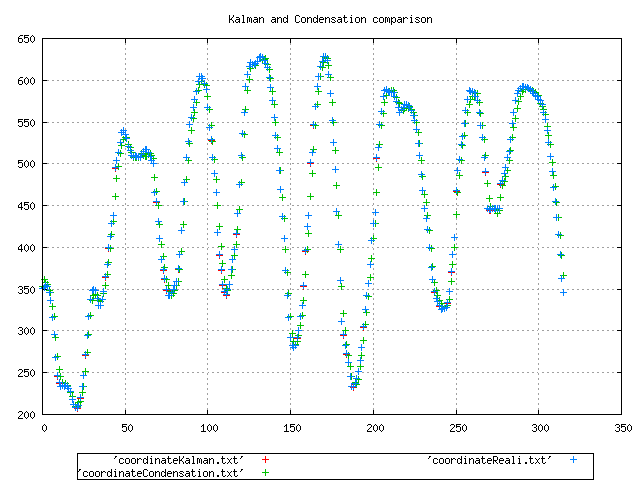
\includegraphics[scale=0.1]{../esperimenti/movie12/mod_3-Q_2000-S_1000/plot.png}\\
% 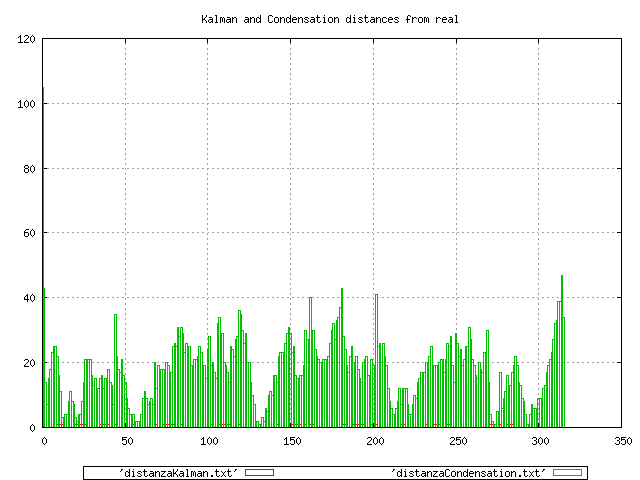
\includegraphics[scale=0.1]{../esperimenti/movie12/mod_3-Q_2000-S_1000/plot-distances.png}
% 
% \column{.20\textwidth}
% \begin{scriptsize}
% \begin{itemize}
% \item [M]3
% \item [Q]1000
% \item [S]5000
% \end{itemize}
% \end{scriptsize}
% 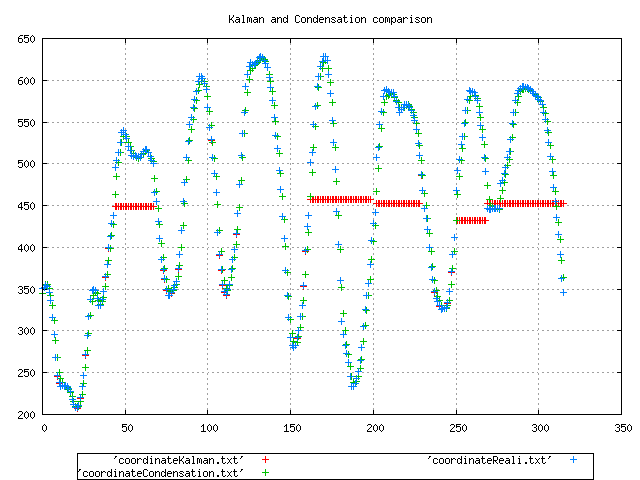
\includegraphics[scale=0.1]{../esperimenti/movie12/mod_3-Q_1000-S_5000/plot.png}\\
% 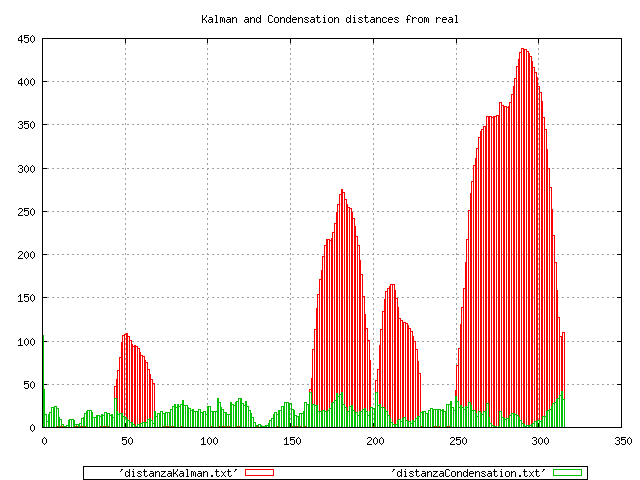
\includegraphics[scale=0.1]{../esperimenti/movie12/mod_3-Q_1000-S_5000/plot-distances.png}
% 
% \column{.20\textwidth}
% \begin{scriptsize}
% \begin{itemize}
% \item [M]3
% \item [Q]1000
% \item [S]100
% \end{itemize}
% \end{scriptsize}
% 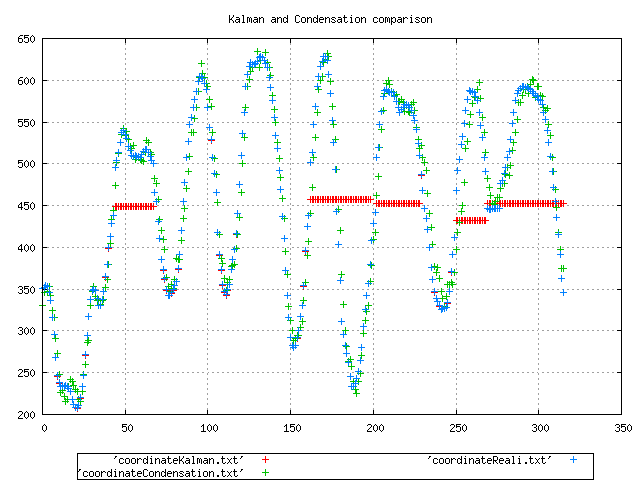
\includegraphics[scale=0.1]{../esperimenti/movie12/mod_3-Q_1000-S_100/plot.png}\\
% 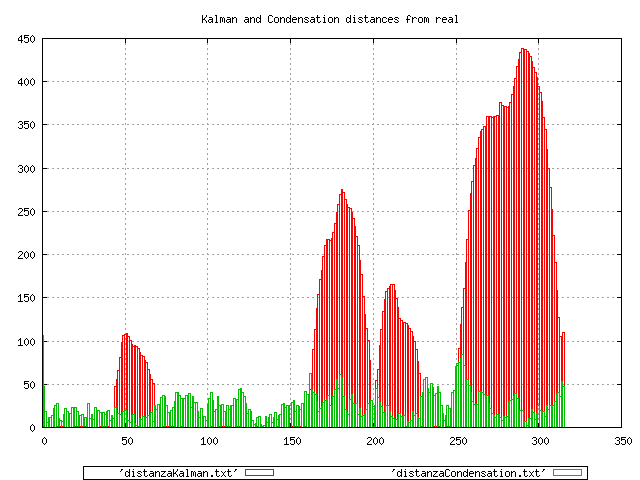
\includegraphics[scale=0.1]{../esperimenti/movie12/mod_3-Q_1000-S_100/plot-distances.png}
% \end{columns}
% 
% }
% %%%%%%%%%%%%%%%%%%%%%%%%%%%%%%%%%%%%%%%%%%
% \frame{\frametitle{Secondo video - tappetonozoom.avi}
% \begin{columns}
% \column{.65\textwidth}
% \begin{small}\begin{itemize}
%  \item moto vario, repentine accelerazioni, oggetto entra ed esce dalla scena
% \item 320x240, 10$fps$, 59$s$
% \end{itemize}\end{small}
% 
% \column{.35\textwidth}\centering
% 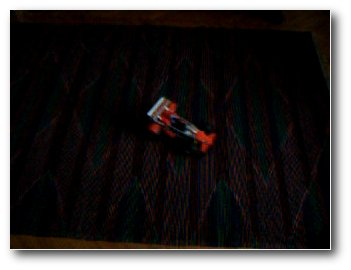
\includegraphics[scale=0.25]{../relazione/figure/tappeto_nozoom.jpg}
% \end{columns}
% \begin{columns}
% 
% \column{.20\textwidth}
% \begin{scriptsize}
% \begin{itemize}
% \item [M]3
% \item [Q]1000
% \item [S]1000
% \end{itemize}
% \end{scriptsize}
% 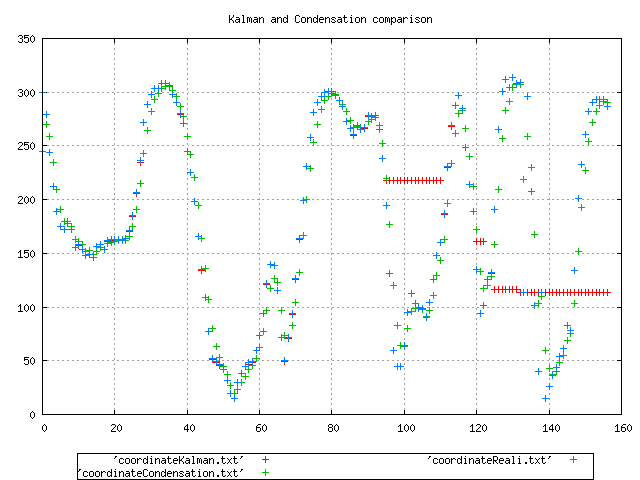
\includegraphics[scale=0.1]{../esperimenti/tappeto_nozoom/mod_3-Q_1000-S_1000/plot.png}\\
% 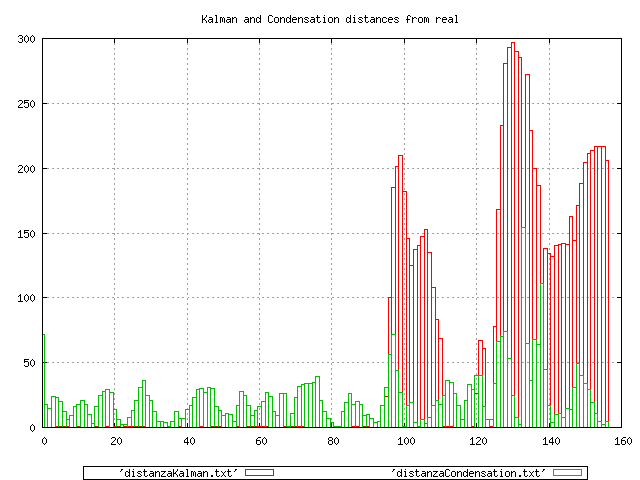
\includegraphics[scale=0.1]{../esperimenti/tappeto_nozoom/mod_3-Q_1000-S_1000/plot-distances.png}
% 
% \column{.20\textwidth}
% \begin{scriptsize}
% \begin{itemize}
% \item [M]5
% \item [Q]1000
% \item [S]1000
% \end{itemize}
% \end{scriptsize}
% 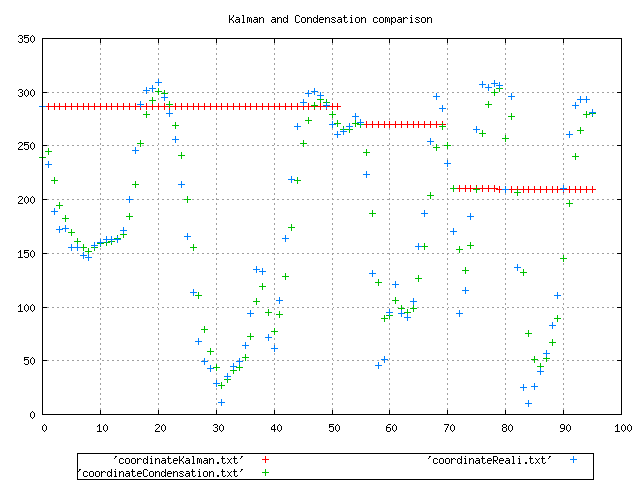
\includegraphics[scale=0.1]{../esperimenti/tappeto_nozoom/mod_5-Q_1000-S_1000/plot.png}\\
% 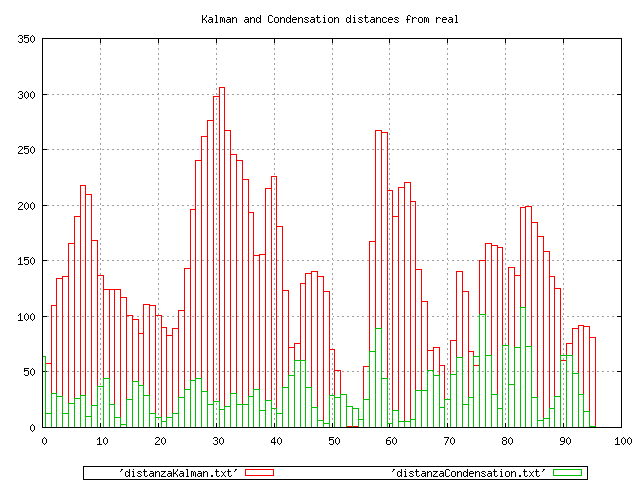
\includegraphics[scale=0.1]{../esperimenti/tappeto_nozoom/mod_5-Q_1000-S_1000/plot-distances.png}
% 
% 
% \column{.20\textwidth}
% \begin{scriptsize}
% \begin{itemize}
% \item [M]2
% \item [Q]1000
% \item [S]1000
% \end{itemize}
% \end{scriptsize}
% 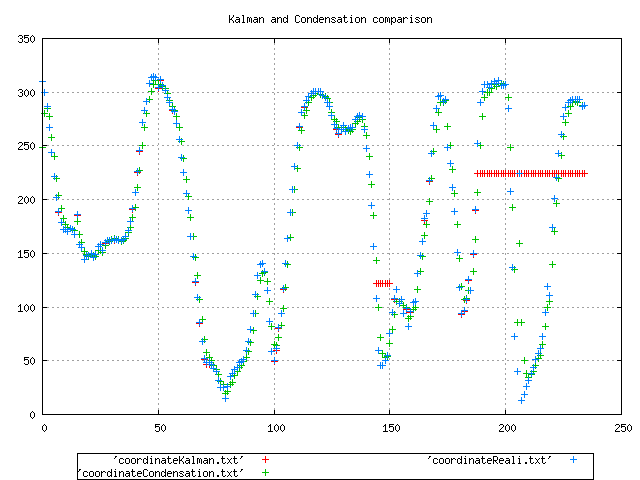
\includegraphics[scale=0.1]{../esperimenti/tappeto_nozoom/mod_2-Q_1000-S_1000/plot.png}\\
% 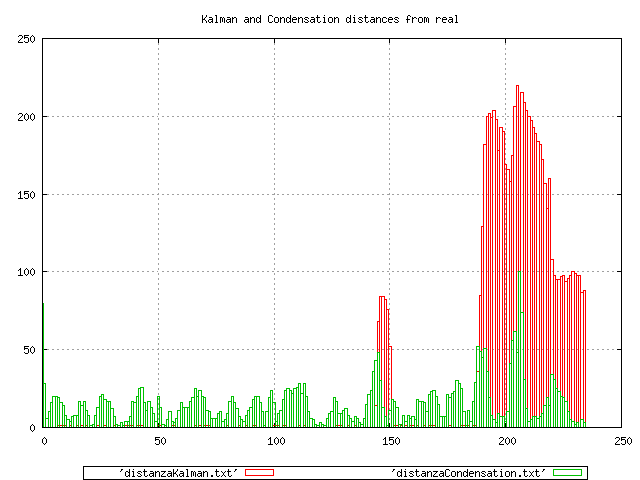
\includegraphics[scale=0.1]{../esperimenti/tappeto_nozoom/mod_2-Q_1000-S_1000/plot-distances.png}
% 
% 
% \column{.20\textwidth}
% \begin{scriptsize}
% \begin{itemize}
% \item [M]1
% \item [Q]2000
% \item [S]1000
% \end{itemize}
% \end{scriptsize}
% 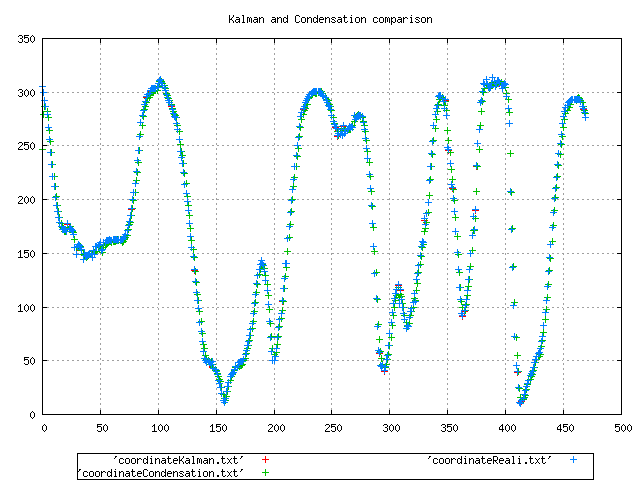
\includegraphics[scale=0.1]{../esperimenti/tappeto_nozoom/mod_1-Q_2000-S_1000/plot.png}\\
% 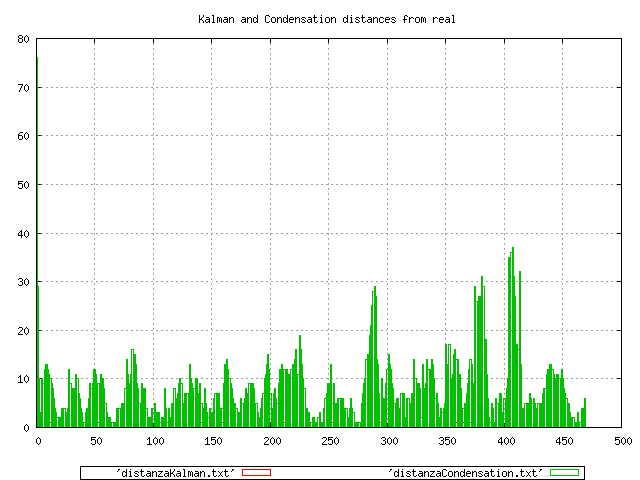
\includegraphics[scale=0.1]{../esperimenti/tappeto_nozoom/mod_1-Q_2000-S_1000/plot-distances.png}
% \end{columns}
% 
% }
% %%%%%%%%%%%%%%%%%%%%%%%%%%%%%%%%%%%%%%%%%%
% \frame{\frametitle{Terzo video - singlecar.avi}
% \begin{columns}
% \column{.65\textwidth}
% \begin{small}\begin{itemize}
%  \item moto costante, oggetto entra ed esce dalla scena
% \item 648x484, 30$fps$, 33$s$
% \end{itemize}\end{small}
% 
% \column{.35\textwidth}\centering
% 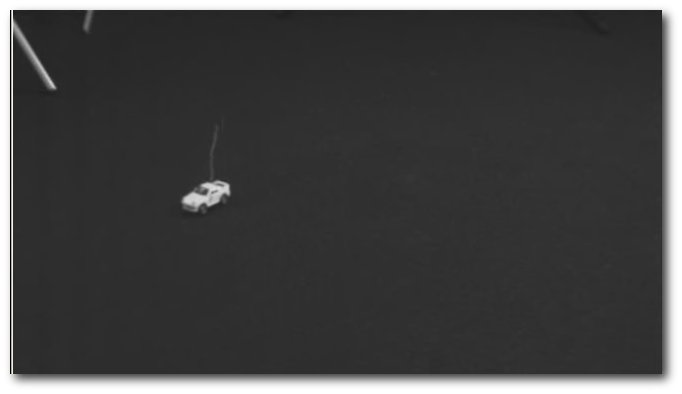
\includegraphics[scale=0.15]{../relazione/figure/singlecar.jpg}
% \end{columns}
% \begin{columns}
% 
% \column{.20\textwidth}
% \begin{scriptsize}
% \begin{itemize}
% \item [M]3
% \item [Q]1000
% \item [S]1000
% \end{itemize}
% \end{scriptsize}
% 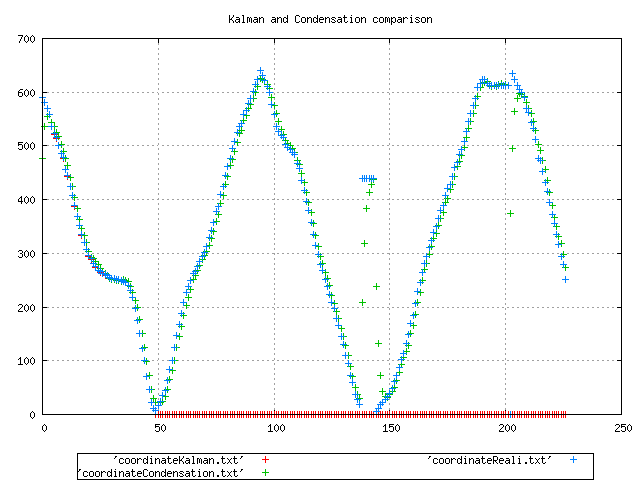
\includegraphics[scale=0.1]{../esperimenti/single_car/mod_3-Q_1000-S_1000/plot.png}\\
% 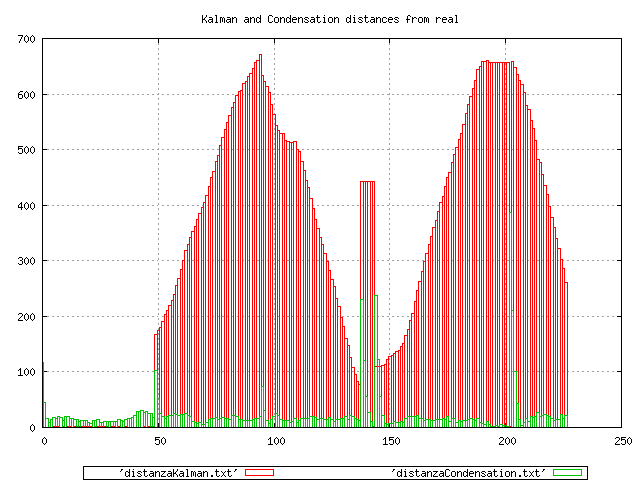
\includegraphics[scale=0.1]{../esperimenti/single_car/mod_3-Q_1000-S_1000/plot-distances.png}
% 
% \column{.20\textwidth}
% \begin{scriptsize}
% \begin{itemize}
% \item [M]10
% \item [Q]5000
% \item [S]1000
% \end{itemize}
% \end{scriptsize}
% 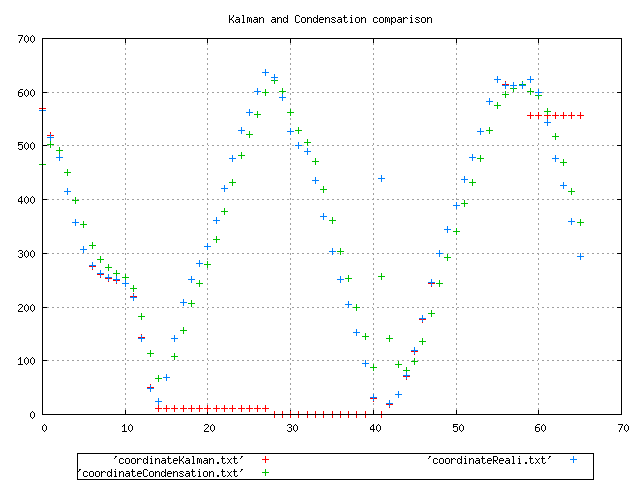
\includegraphics[scale=0.1]{../esperimenti/single_car/mod_10-Q_5000-S_1000/plot.png}\\
% 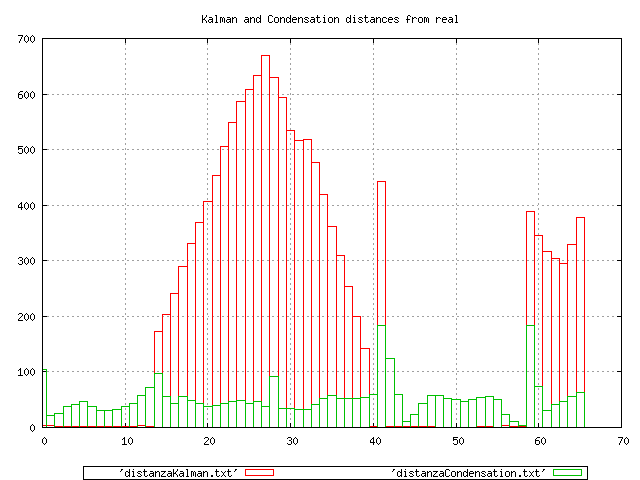
\includegraphics[scale=0.1]{../esperimenti/single_car/mod_10-Q_5000-S_1000/plot-distances.png}
% 
% \column{.20\textwidth}
% \begin{scriptsize}
% \begin{itemize}
% \item [M]6
% \item [Q]0.1
% \item [S]1000
% \end{itemize}
% \end{scriptsize}
% 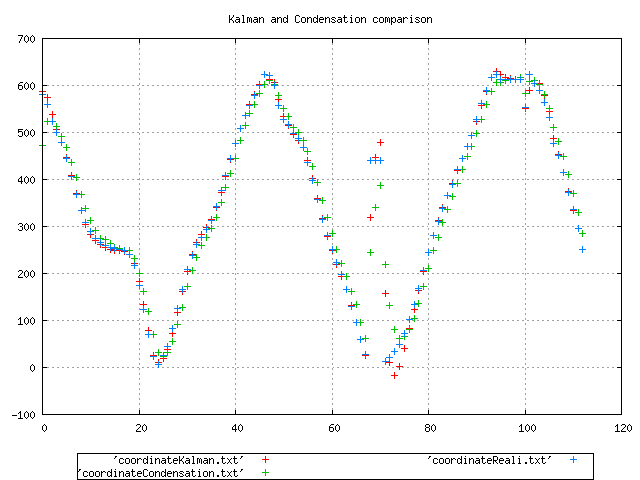
\includegraphics[scale=0.1]{../esperimenti/single_car/mod_6-Q_0.1-S_1000/plot.png}\\
% 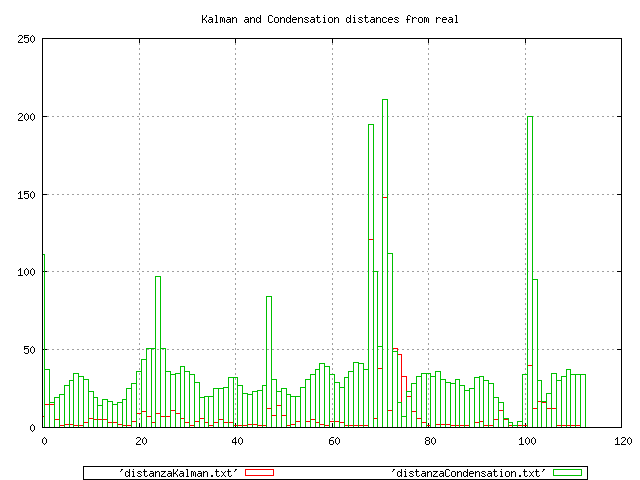
\includegraphics[scale=0.1]{../esperimenti/single_car/mod_6-Q_0.1-S_1000/plot-distances.png}
% 
% \column{.20\textwidth}
% \begin{scriptsize}
% \begin{itemize}
% \item [M]1
% \item [Q]0.0001
% \item [S]1000
% \end{itemize}
% \end{scriptsize}
% 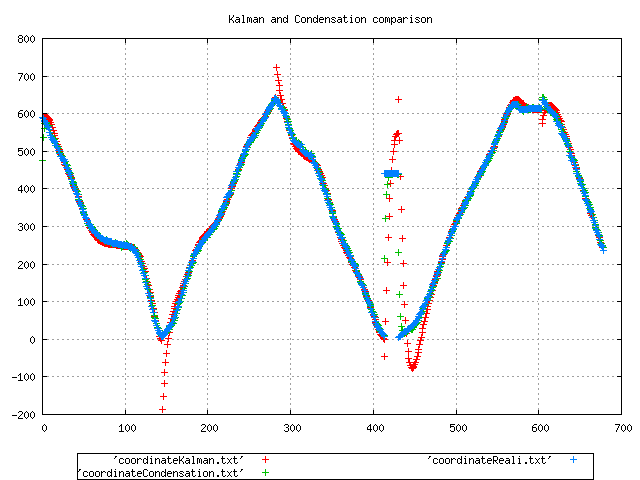
\includegraphics[scale=0.1]{../esperimenti/single_car/mod_1-Q_0.0001-S_1000/plot.png}\\
% 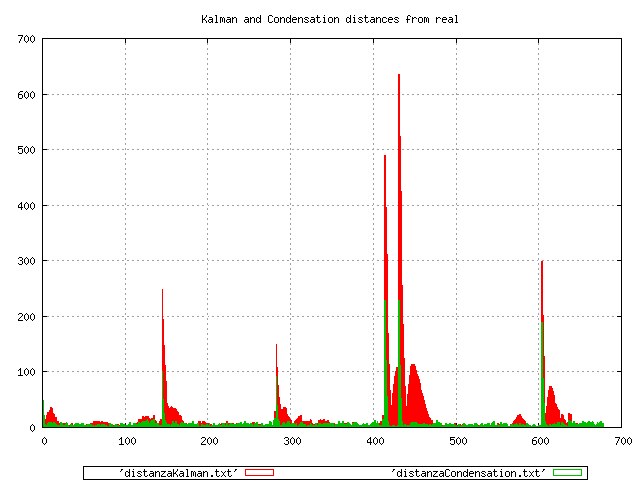
\includegraphics[scale=0.1]{../esperimenti/single_car/mod_1-Q_0.0001-S_1000/plot-distances.png}
% \end{columns}
% }
%%%%%%%%%%%%%%%%%%%%%%%%%%%%%%%%%%%%%%%%%%
\subsection{Risultati}

%%%%%%%%%%%%%%%%%%%%%%%%%%%%%%%%%%%%%%%%%%
\frame{\frametitle{movie12.mjpeg - MOD:3, Q:1000, S:1000}

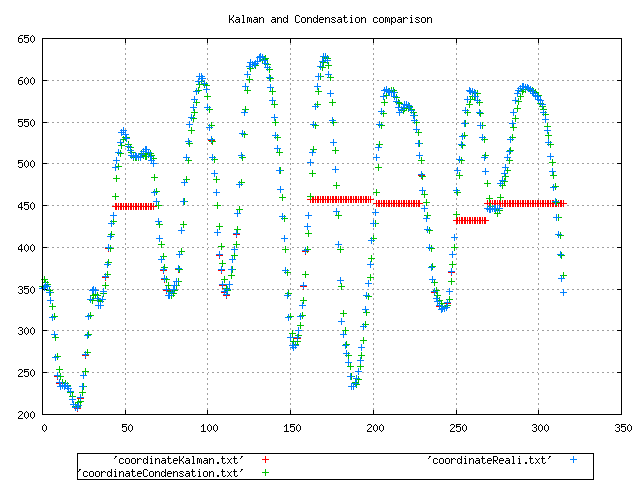
\includegraphics[scale=0.45]{../esperimenti/movie12/mod_3-Q_1000-S_1000/plot.png}

}
%%%%%%%%%%%%%%%%%%%%%%%%%%%%%%%%%%%%%%%%%%
\frame{\frametitle{movie12.mjpeg - MOD:3, Q:1000, S:10}
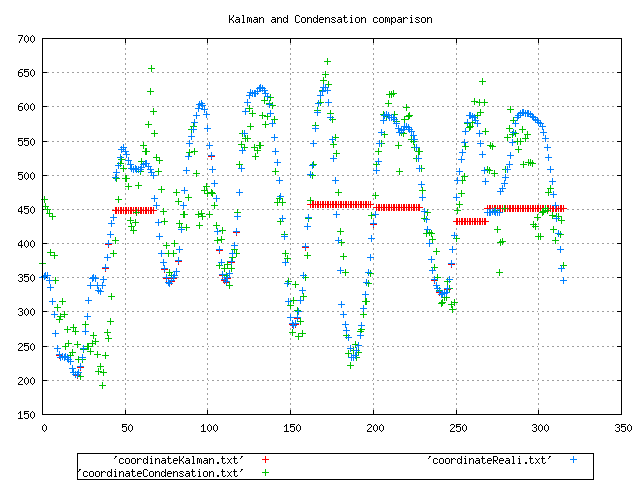
\includegraphics[scale=0.45]{../esperimenti/movie12/mod_3-Q_1000-S_10/plot.png}
}
%%%%%%%%%%%%%%%%%%%%%%%%%%%%%%%%%%%%%%%%%%
\frame{\frametitle{movie12.mjpeg - MOD:3, Q:1000, S:1000}
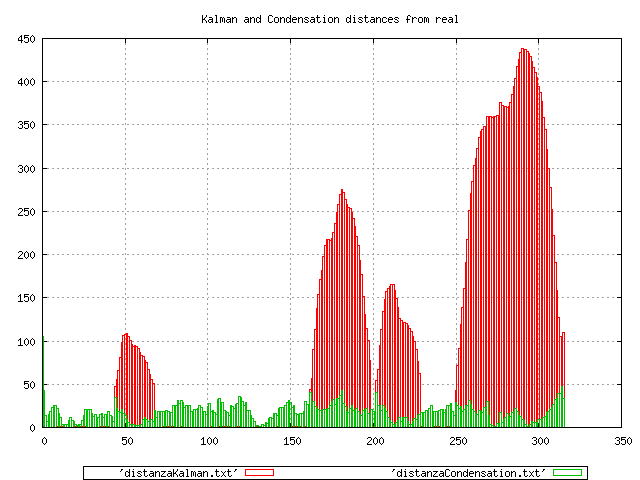
\includegraphics[scale=0.45]{../esperimenti/movie12/mod_3-Q_1000-S_1000/plot-distances.png}
}
%%%%%%%%%%%%%%%%%%%%%%%%%%%%%%%%%%%%%%%%%%
\frame{\frametitle{movie12.mjpeg - MOD:3, Q:1000, S:10}
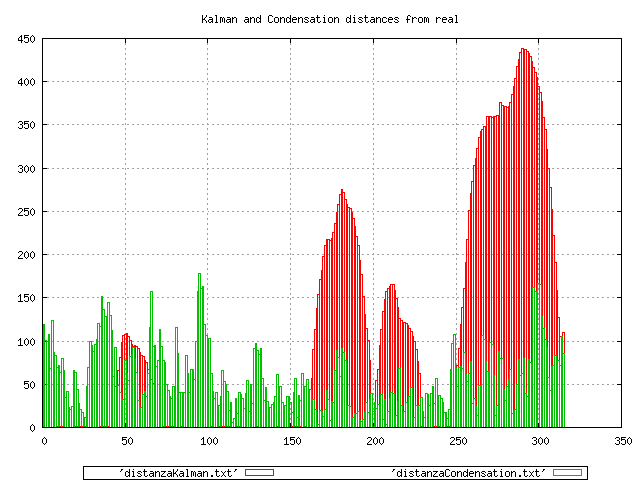
\includegraphics[scale=0.45]{../esperimenti/movie12/mod_3-Q_1000-S_10/plot-distances.png}
}


% 
%%%%%%%%%%%%%%%%%%%%%%%%%%%%%%%%%%%%%%%%%%
\frame{\frametitle{tappetonozoom.avi - MOD:2, Q:1000, S:1000}
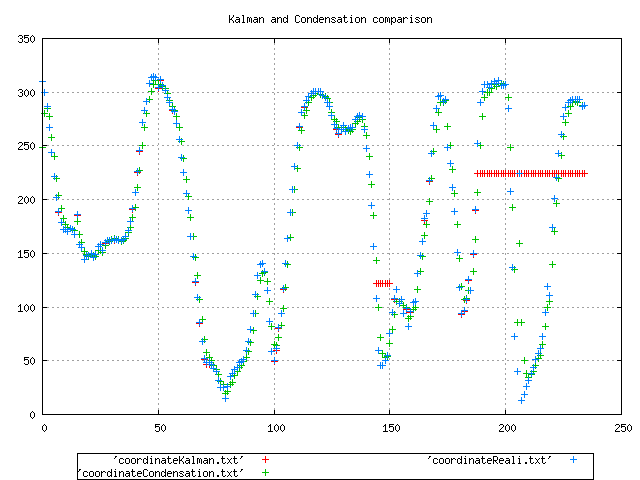
\includegraphics[scale=0.45]{../esperimenti/tappeto_nozoom/mod_2-Q_1000-S_1000/plot.png}
}
%%%%%%%%%%%%%%%%%%%%%%%%%%%%%%%%%%%%%%%%%%
\frame{\frametitle{tappetonozoom.avi - MOD:1, Q:500, S:10}
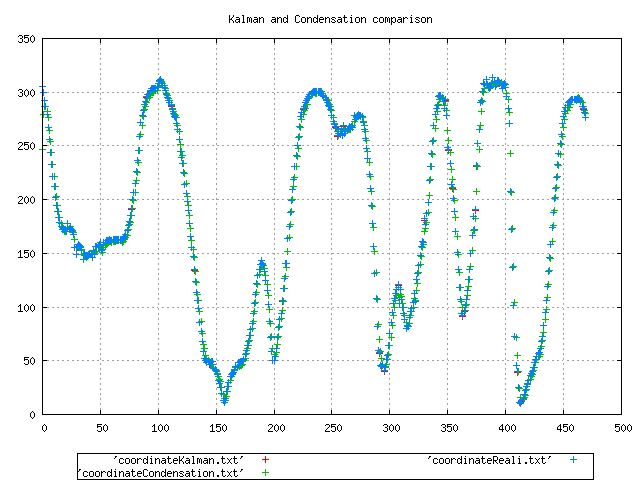
\includegraphics[scale=0.45]{../esperimenti/tappeto_nozoom/mod_1-Q_500-S_1000/plot.png}
}
%%%%%%%%%%%%%%%%%%%%%%%%%%%%%%%%%%%%%%%%%%
\frame{\frametitle{tappetonozoom.avi - MOD:2, Q:1000, S:1000}
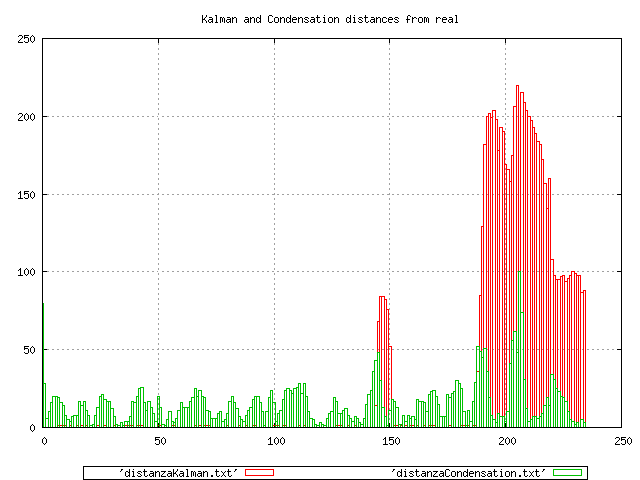
\includegraphics[scale=0.45]{../esperimenti/tappeto_nozoom/mod_2-Q_1000-S_1000/plot-distances.png}
}
%%%%%%%%%%%%%%%%%%%%%%%%%%%%%%%%%%%%%%%%%%
\frame{\frametitle{tappetonozoom.avi - MOD:1, Q:500, S:10}
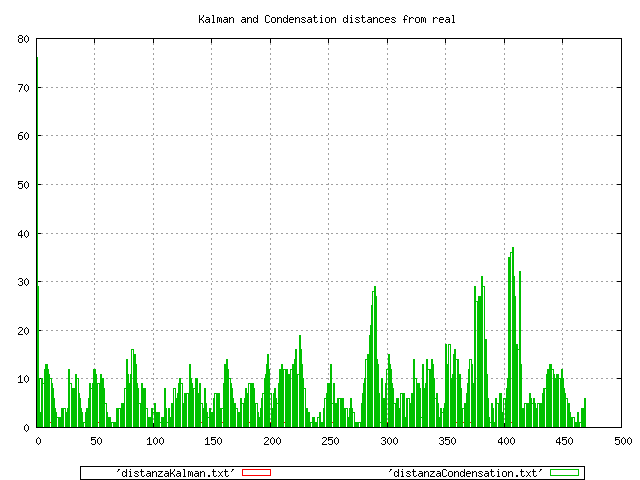
\includegraphics[scale=0.45]{../esperimenti/tappeto_nozoom/mod_1-Q_500-S_1000/plot-distances.png}
}


% 
%%%%%%%%%%%%%%%%%%%%%%%%%%%%%%%%%%%%%%%%%%
\frame{\frametitle{tappetonozoom.avi - MOD:1, Q:1, S:1000}
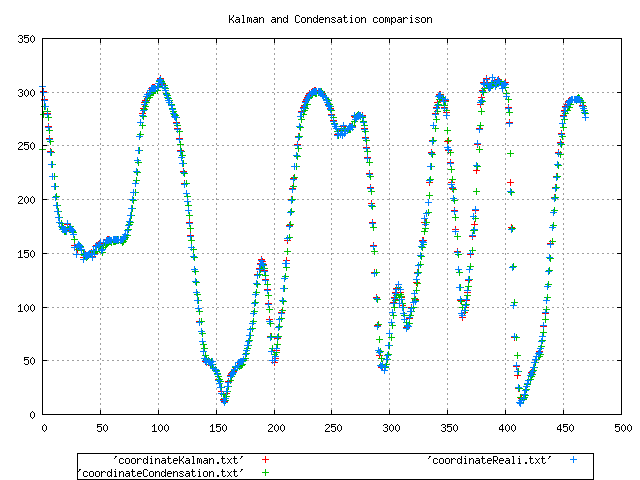
\includegraphics[scale=0.45]{../esperimenti/tappeto_nozoom/mod_1-Q_1-S_1000/plot.png}
}
%%%%%%%%%%%%%%%%%%%%%%%%%%%%%%%%%%%%%%%%%%
\frame{\frametitle{tappetonozoom.avi - MOD:1, Q:0.001, S:1000}
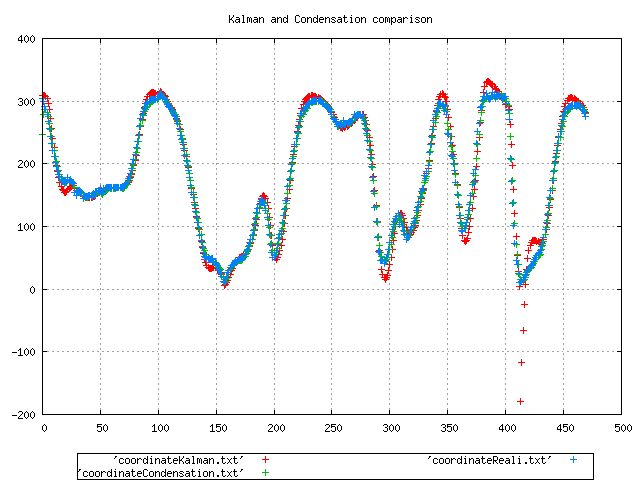
\includegraphics[scale=0.45]{../esperimenti/tappeto_nozoom/mod_1-Q_0.001-S_1000/plot.png}
}
%%%%%%%%%%%%%%%%%%%%%%%%%%%%%%%%%%%%%%%%%%
\frame{\frametitle{tappetonozoom.avi - MOD:1, Q:1, S:1000}
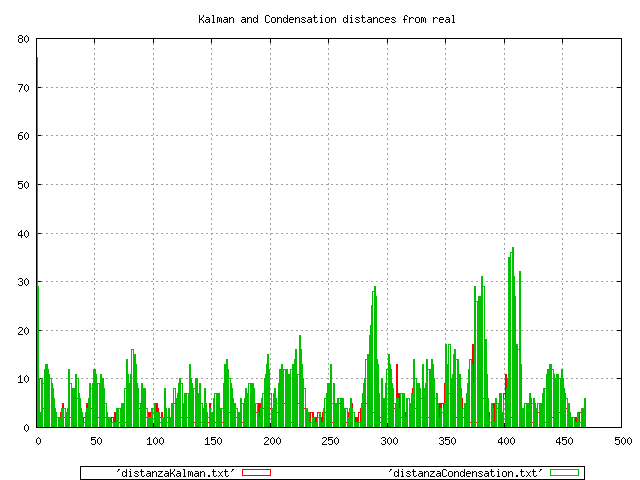
\includegraphics[scale=0.45]{../esperimenti/tappeto_nozoom/mod_1-Q_1-S_1000/plot-distances.png}
}
%%%%%%%%%%%%%%%%%%%%%%%%%%%%%%%%%%%%%%%%%%
\frame{\frametitle{tappetonozoom.avi - MOD:1, Q:0.001, S:1000}
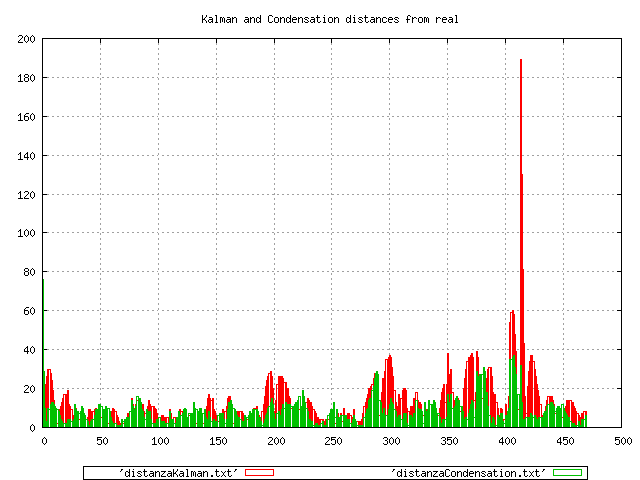
\includegraphics[scale=0.45]{../esperimenti/tappeto_nozoom/mod_1-Q_0.001-S_1000/plot-distances.png}
}